% !Rnw weave = knitr
\documentclass[dvipsnames]{beamer}\usepackage[]{graphicx}\usepackage[]{color}
%% maxwidth is the original width if it is less than linewidth
%% otherwise use linewidth (to make sure the graphics do not exceed the margin)
\makeatletter
\def\maxwidth{ %
  \ifdim\Gin@nat@width>\linewidth
    \linewidth
  \else
    \Gin@nat@width
  \fi
}
\makeatother

\definecolor{fgcolor}{rgb}{0.345, 0.345, 0.345}
\newcommand{\hlnum}[1]{\textcolor[rgb]{0.686,0.059,0.569}{#1}}%
\newcommand{\hlstr}[1]{\textcolor[rgb]{0.192,0.494,0.8}{#1}}%
\newcommand{\hlcom}[1]{\textcolor[rgb]{0.678,0.584,0.686}{\textit{#1}}}%
\newcommand{\hlopt}[1]{\textcolor[rgb]{0,0,0}{#1}}%
\newcommand{\hlstd}[1]{\textcolor[rgb]{0.345,0.345,0.345}{#1}}%
\newcommand{\hlkwa}[1]{\textcolor[rgb]{0.161,0.373,0.58}{\textbf{#1}}}%
\newcommand{\hlkwb}[1]{\textcolor[rgb]{0.69,0.353,0.396}{#1}}%
\newcommand{\hlkwc}[1]{\textcolor[rgb]{0.333,0.667,0.333}{#1}}%
\newcommand{\hlkwd}[1]{\textcolor[rgb]{0.737,0.353,0.396}{\textbf{#1}}}%
\let\hlipl\hlkwb

\usepackage{framed}
\makeatletter
\newenvironment{kframe}{%
 \def\at@end@of@kframe{}%
 \ifinner\ifhmode%
  \def\at@end@of@kframe{\end{minipage}}%
  \begin{minipage}{\columnwidth}%
 \fi\fi%
 \def\FrameCommand##1{\hskip\@totalleftmargin \hskip-\fboxsep
 \colorbox{shadecolor}{##1}\hskip-\fboxsep
     % There is no \\@totalrightmargin, so:
     \hskip-\linewidth \hskip-\@totalleftmargin \hskip\columnwidth}%
 \MakeFramed {\advance\hsize-\width
   \@totalleftmargin\z@ \linewidth\hsize
   \@setminipage}}%
 {\par\unskip\endMakeFramed%
 \at@end@of@kframe}
\makeatother

\definecolor{shadecolor}{rgb}{.97, .97, .97}
\definecolor{messagecolor}{rgb}{0, 0, 0}
\definecolor{warningcolor}{rgb}{1, 0, 1}
\definecolor{errorcolor}{rgb}{1, 0, 0}
\newenvironment{knitrout}{}{} % an empty environment to be redefined in TeX

\usepackage{alltt}

%%%%%%%%%%%%
% Packages %
%%%%%%%%%%%%

\usepackage[]{hyperref} % Links, pretty and functional
\usepackage{listings} % Prettier code blocks
\usepackage{graphicx} % Include graphics
\usepackage{multicol} % Columns
\usepackage{tikz-qtree,tikz-qtree-compat} % Syntax trees
\tikzset{every tree node/.style={align=center,anchor=north}}
\usepackage{amsmath,amssymb,stmaryrd} % Mathy symbols for semantics
\usepackage{gb4e} % Glossing. MUST BE LAST PACKAGE LOADED.
\resetcounteronoverlays{exx} % Fixes weird beamer exe numbering issue

%%%%%%%%%%%%
% Settings %
%%%%%%%%%%%%

% Beamer settings
\usetheme[]{Singapore} % http://deic.uab.es/~iblanes/beamer_gallery/
\usecolortheme{dove}
\usefonttheme{serif}

\renewcommand{\insertnavigation}[1]{}
\setbeamertemplate{navigation symbols}{}

\setbeamertemplate{section in toc}[sections numbered] %This enumerates the tables of contents
\AtBeginSection[]
{
	\begin{frame}
		\frametitle{}
		\tableofcontents[currentsection]
	\end{frame}
} % This reproduces the table of contents before each section, with just the current section highlighted. 

% Listings and color settings
\definecolor{mygray}{gray}{0.95}
\lstdefinestyle{mystyle}{
    backgroundcolor=\color{mygray},   
    commentstyle=\color{darkgray},
    keywordstyle=\color{red},
    numberstyle=\small\color{darkgray},
    stringstyle=\color{purple},
    basicstyle=\ttfamily\small,
    breakatwhitespace=false,         
    breaklines=true,   
    keepspaces=true,                 
    numbers=left,                    
    numbersep=5pt,
    tabsize=2
}
 
\lstset{style=mystyle}

% Commands
\newcommand{\type}[1]{\ensuremath{\langle #1 \rangle}}
\newcommand{\denote}[1]{\ensuremath{\llbracket \text{#1} \rrbracket}}

%%%%%%%%%%%%%%%%%%
% Titlepage info %
%%%%%%%%%%%%%%%%%%

\title{R + \LaTeX\ = knitr}
\author[Cara Feldscher]{Cara Feldscher\\\href{mailto:feldsch3@msu.edu}{feldsch3@msu.edu}}
\institute[Michigan State University]{Michigan State University}
\date{ R-Ladies \\ \today}

\logo{
\includegraphics[height=1.5cm]{rladies-basic-logo1.pdf}}

%%%%%%
\IfFileExists{upquote.sty}{\usepackage{upquote}}{}
\begin{document}

\maketitle

%

\section{Why I care about R}

\begin{frame}[fragile] % If you include a verbatim environment, you need the fragile option because https://pbelmans.ncag.info/blog/2011/02/20/why-latex-beamer-needs-fragile-when-using-verbatim/
  \frametitle{Why I care about R}
  
  Actually, I don't think I need to answer this!
  
\end{frame}

%

\section{Why I care about \LaTeX}

\begin{frame}[fragile]
  \frametitle{Subfield secret handshakes}
    
    \begin{exe}
      \ex ~ \vspace{-1em}
      
      	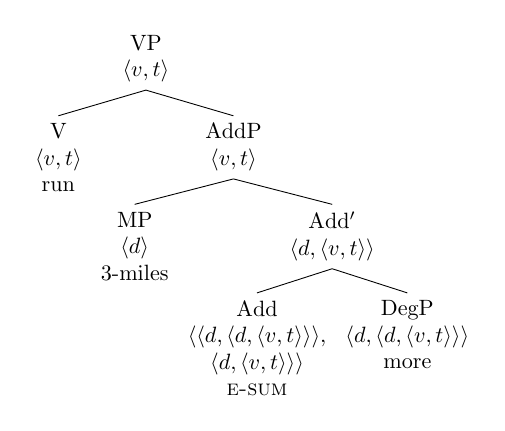
\begin{tikzpicture}[scale=.8]
        	\tikzset{level distance=40pt}
        	\Tree
          [.VP\\$\type{v,t}$ [.V\\$\type{v,t}$\\run ] [.AddP\\$\type{v,t}$ [.MP\\$\type{d}$\\3-miles ] [.Add$'$\\$\type{d,\type{v,t}}$ [.Add\\$\langle\type{d,\type{d,\type{v,t}}},$\\$\type{d,\type{v,t}}\rangle$\\\textsc{e-sum} ] [.DegP\\$\type{d,\type{d,\type{v,t}}}$\\more ] ] ] ]
      	\end{tikzpicture}	
	
      \ex $\llbracket\textsc{e-sum}_v\rrbracket = \lambda f_{\type{d,\type{d,\type{v,t}}}} \lambda d \lambda v' 
	          \left[
	          \begin{array}{l}
	            \mu (v') = d \wedge\\
	            f(\mu(v))(d)(v \oplus v')
	          \end{array}
	          \right]$
    \end{exe}
\end{frame}

%

\begin{frame}[fragile]
  \frametitle{Control, flexibility, convenience}
    
    There's a package for that.\pause
    
    \begin{lstlisting}[language=TeX]
      \usepackage{hyperref} % Links, pretty and functional
      \usepackage{listings} % Prettier code blocks
      \usepackage{tikz-qtree,tikz-qtree-compat} % Syntax trees
      \usepackage{amsmath,amssymb,stmaryrd} % Mathy symbols for semantics \end{lstlisting}
    % Ended on same line instead of next because it was giving me an extra line in the listing otherwise...

  
\end{frame}

%

\begin{frame}[fragile]
  \frametitle{Control, flexibility, convenience}
  
  Write your own commands.\pause
  
  \begin{lstlisting}[language=TeX]
    % The standard way to note a denotation
    \newcommand{\denotation}[1]{\ensuremath{\llbracket \text{#1} \rrbracket}} 
    
    \denotation{cat} \end{lstlisting}
  % Ended on same line instead of next because it was giving me an extra line in the listing otherwise...
  
  
  \newcommand{\denotation}[1]{\ensuremath{\llbracket \text{#1} \rrbracket = }}
  \begin{exe}
    \ex $\denotation{cat} ...$
  \end{exe}
  
\end{frame}

%

\begin{frame}[fragile]
  \frametitle{Control, flexibility, convenience}
  
  Automated:\pause
  \begin{itemize}
    \item Bibliography and citations
    \item Labeling and referencing (figures, examples, sections, etc.)
    \item Commands 
  \end{itemize}
  
\end{frame}

%

\section{How to use knitr}

%

\begin{frame}[fragile]
  \frametitle{Minimal Working Example 1}
  
\begin{knitrout}\tiny
\definecolor{shadecolor}{rgb}{0.969, 0.969, 0.969}\color{fgcolor}\begin{kframe}
\begin{alltt}
\hlkwd{library}\hlstd{(ggplot2)}
\hlkwd{data}\hlstd{(}\hlstr{"mtcars"}\hlstd{)}
\hlcom{# Is there a relationship between displacement and HP?}
\hlkwd{ggplot}\hlstd{(mtcars,} \hlkwd{aes}\hlstd{(}\hlkwc{x}\hlstd{=disp,} \hlkwc{y}\hlstd{=hp))} \hlopt{+}
\hlkwd{geom_point}\hlstd{()}\hlopt{+}
\hlkwd{geom_smooth}\hlstd{(}\hlkwc{method} \hlstd{=} \hlstr{"lm"}\hlstd{)}
\end{alltt}
\end{kframe}
\includegraphics[width=\maxwidth]{figure/data1-1} 

\end{knitrout}
    
    \begin{itemize}
      \item \verb echo = TRUE
      \item \verb eval = TRUE
    \end{itemize}
        
\end{frame}

%

\begin{frame}[fragile]
  \frametitle{Minimal Working Example 2}
  
\begin{knitrout}\tiny
\definecolor{shadecolor}{rgb}{0.969, 0.969, 0.969}\color{fgcolor}
\includegraphics[width=\maxwidth]{figure/data2-1} 

\end{knitrout}
    
    \begin{itemize}
      \item \verb echo = FALSE
      \item \verb eval = TRUE
    \end{itemize}
        
\end{frame}

%

\begin{frame}[fragile]
  \frametitle{Minimal Working Example 3}
  
\begin{knitrout}\tiny
\definecolor{shadecolor}{rgb}{0.969, 0.969, 0.969}\color{fgcolor}\begin{kframe}
\begin{alltt}
\hlkwd{library}\hlstd{(ggplot2)}
\hlkwd{data}\hlstd{(}\hlstr{"mtcars"}\hlstd{)}
\hlcom{# Is there a relationship between displacement and HP?}
\hlkwd{ggplot}\hlstd{(mtcars,} \hlkwd{aes}\hlstd{(}\hlkwc{x}\hlstd{=disp,} \hlkwc{y}\hlstd{=hp))} \hlopt{+}
\hlkwd{geom_point}\hlstd{()}\hlopt{+}
\hlkwd{geom_smooth}\hlstd{(}\hlkwc{method} \hlstd{=} \hlstr{"lm"}\hlstd{)}
\end{alltt}
\end{kframe}
\end{knitrout}
    
    \begin{itemize}
      \item \verb echo = TRUE
      \item \verb eval = FALSE
    \end{itemize}
        
\end{frame}

%

\section{Why you might care}

%

\begin{frame}[fragile]
  \frametitle{The code is in your document}
  
  Reproducibility!
  
\end{frame}

%

\begin{frame}[fragile]
  \frametitle{The code is in your document}
  
  Say goodbye to:
  \begin{itemize}
    \item Forgetting to update your graph after you add data.
    \item Grabbing the wrong graph.
    \item Saving over the graph you want.
    \item Copy pasting the wrong graph / code into your paper.
  \end{itemize}
\end{frame}

%

\begin{frame}[fragile]
  \frametitle{The code is in your document}
  
  Display it if you want, not if you don't, and change your mind whenever you want.
  
\end{frame}

%

\begin{frame}[fragile]
  \frametitle{\LaTeX\ is cool}
  
  \LaTeX\ is cool, for all the aforementioned reasons.\pause
  
  ...Or you can use Markdown.
  
\end{frame}

%

\section{Conclusion}

%

\begin{frame}[fragile]
  \frametitle{Conclusion}
  
  Thanks Yihui! (\href{https://yihui.name/knitr/}{\color{violet}website}, \href{https://github.com/yihui/knitr}{\color{violet}github})
  
\end{frame}

%

\begin{frame}[fragile]
  \frametitle{Thanks!}
  
  If you want the slides or code, it's available through R-Ladies, or at \href{https://github.com/cfeldscher}{\color{violet}https://github.com/cfeldscher}.
  
  Set up instructions follow in an appendix slide.
  
\end{frame}

%

\section*{Appendix - set up}

%

\begin{frame}
  \frametitle{Knitr set-up}
  
  \begin{multicols}{2}
  \begin{enumerate}
    \item Install package \texttt{knitr}
    \item Change default from sweave to knitr in the global settings:
    \item Create a wholly \LaTeX\ (or Markdown) document in RStudio.
    \item Where you want R code, insert a code block.
    \item If you're iffy on the above two steps, look at the code for this doc.
  \end{enumerate}
  
  \columnbreak
  
  \includegraphics[height=2in]{knitr-settings-crop.png}
  \end{multicols}
  
\end{frame}

%

\begin{frame}
  \frametitle{\LaTeX\ resources}
  
  Installing: \href{https://www.latex-project.org/get/}{\color{violet}https://www.latex-project.org/get/}
  \vspace{2em}
  
  Other potential resources:
  \begin{itemize}
    \item \href{https://www.sharelatex.com/blog/latex-guides/beginners-tutorial.html}{\color{violet}https://www.sharelatex.com/blog/latex-guides/beginners-tutorial.html}\footnote{I haven't actually checked these out, but I've found ShareLatex's overviews of packages and such very clear and helpful.}
    \item \href{https://tex.stackexchange.com/}{\color{violet}https://tex.stackexchange.com/}
  \end{itemize}
\end{frame}

%

\begin{frame}
  \frametitle{Workflow suggestions}
  
  Knitr compiles pretty slowly. This should be your final document, not your testing and exploring data document. Do all that in a different R file, then put the important stuff in a knitr file. Additionally, RStudio doesn't have the \LaTeX\ spellcheck or autocomplete that your usual \TeX\ editor might have, so you should either proofread carefully, or check it in a tex editor.
  
\end{frame}




\end{document}
